% ============================================================================
%  Physical Review B -- version v2
%  Emergent altermagnetic correlations and d_xy pairing in the checkerboard
%  Hubbard model
%
%  Every number in this file traces to a file in the repository. Pointers are
%  given in comments beside each claim so the draft can be checked against data
%  rather than against memory. Items still needing input are marked TODO.
% ============================================================================
\documentclass[aps,prb,reprint,superscriptaddress,amsmath,amssymb,floatfix]{revtex4-2}

\usepackage{graphicx}
\usepackage{bm}

\renewcommand{\topfraction}{0.9}
\renewcommand{\bottomfraction}{0.8}
\renewcommand{\textfraction}{0.07}
\renewcommand{\floatpagefraction}{0.7}
\setcounter{topnumber}{3}
\setcounter{totalnumber}{4}

\begin{document}

\title{Interaction-induced $d_{xy}$ pairing in the checkerboard Hubbard model}

% TODO: author list and affiliations to be completed by the authors.
\author{[Author One]}
\affiliation{[Affiliation]}
\author{[Author Two]}
\affiliation{[Affiliation]}

\date{\today}

\begin{abstract}
We compute the pair-field vertex of the half-filled Hubbard model on the
checkerboard lattice by constrained-path quantum Monte Carlo on lattices of
$8\times8$, $10\times10$ and $12\times12$ sites. Separating the
interaction-induced vertex from the uncorrelated part of the correlator, we find
that the vertex vanishes identically in all four channels at $U=0$, so every
feature reported here is generated by the interaction. The on-site $s$ vertex is
negative throughout, as a repulsive interaction requires. The leading
sign-changing channel changes with the lattice anisotropy $\delta$, from
extended $s$ at small $\delta$ to $d_{xy}$ above a crossover $\delta_c$. That
crossover is nearly independent of the interaction strength and its spread
across $U$ narrows from $0.148$ to $0.028$ between $L=8$ and $L=12$, converging
on $\delta_c \simeq 0.19$, which identifies it as a property of the lattice
geometry. The $d_{xy}$ vertex grows with system size by a factor between $2.18$
and $2.38$ over the same range, and $d_{x^2-y^2}$ is positive in all 126 cells
examined. The dominant channel lies outside the pairing basis used in earlier
work on this lattice.
\end{abstract}

\maketitle


% -------------------------------------------------------------------------
\section{Introduction}
% ---------------------------------------------------------------------------

Altermagnets combine a vanishing net moment with a spin-split band structure,
a combination long assumed to require either ferromagnetism or spin-orbit
coupling~\cite{Smejkal2022a,Smejkal2022b}. The splitting follows from the
crystal symmetry: the two opposite-spin sublattices are connected by a rotation
rather than by a translation or an inversion, so the spin degeneracy that a
conventional antiferromagnet enforces is absent.

Most microscopic models of this state build the splitting into the Hamiltonian,
usually through a spin-dependent hopping. The splitting is then present already
at zero interaction and the question of whether interactions alone can produce
it is left open. Two recent studies of the Lieb lattice state the gap directly,
noting that unbiased studies establishing an altermagnet as the ground state of
an interacting Hamiltonian are lacking~\cite{Kaushal2025,Duerrnagel2025}. Both
use methods with a controlled range of validity, unrestricted Hartree-Fock with
exact diagonalization on small clusters in the first case and a functional
renormalization group treatment of the weak-coupling limit in the second.

The checkerboard lattice offers a route to the same physics without putting it
in by hand. It is a square lattice with diagonal bonds on alternating
plaquettes, so the two sublattices are exchanged by a fourfold rotation about a
plaquette center but by no translation. The hopping is spin independent, and
the interaction is a uniform on-site Hubbard $U$. Any spin splitting therefore
appears only once magnetic correlations develop, which is the emergent route
rather than the built-in one.

We report constrained-path quantum Monte Carlo (CPQMC) calculations of the
pair-field vertex for this model at half filling on lattices of $8\times8$,
$10\times10$ and $12\times12$ sites. The vertex is the part of the pair
correlator that the interaction builds, and it is the quantity that distinguishes
a pairing tendency from the large positive correlator that free electrons already
carry. Three results follow. The vertex is zero in every channel at $U=0$. The
leading sign-changing channel is $d_{xy}$ above an anisotropy $\delta_c$ whose
value converges with system size. The $d_{xy}$ vertex grows with system size at
every interaction strength studied, while $d_{x^2-y^2}$ remains positive
throughout and is never repulsive.


% -------------------------------------------------------------------------
\section{Model and method}
% ---------------------------------------------------------------------------

We consider
\begin{equation}
H = \sum_{ij\sigma} t_{ij}\, c^{\dagger}_{i\sigma} c^{\phantom{\dagger}}_{j\sigma}
    + U \sum_i n_{i\uparrow} n_{i\downarrow},
\label{eq:H}
\end{equation}
with nearest-neighbor hopping $t_{ij} = t_0$ and diagonal hopping
$t_1 + t_2$ along $(1,1)$ and $t_1 - t_2$ along $(1,-1)$ on one sublattice, the
two exchanged on the other. Energies are in units of $|t_0|$, and we set
$t_0 = -1$ and $t_1 = 0.3$ throughout. The anisotropy is parametrized by
$\delta$ through $t_2 = -\delta$, so that $\delta = 0$ restores the plain square
lattice with uniform second-neighbor hopping and both sublattices become
equivalent. All calculations are at half filling.

The hopping in Eq.~(\ref{eq:H}) is spin independent by construction, so
$n_{\uparrow}(\bm{k}) = n_{\downarrow}(\bm{k})$ at $U = 0$ for every $\delta$.

We use CPQMC with a Trotter step $\Delta\tau = 0.01$, a projection length
$\beta = 32$, and $N_w = 1000$ walkers. The constrained-path approximation
introduces a bias controlled by the trial wave function, so we do not describe
these results as exact. Doubling the projection length from $\beta = 32$ to
$\beta = 48$ changes the order parameter by between $0.1\%$ and $4.1\%$ with no
systematic drift, which we take as convergence in $\beta$.
% beta convergence: 32 -> 48 changes 0.1, 1.5, 2.4, 4.1 percent

The pair-field correlator is measured in four channels, on-site $s$, extended
$s$, $d_{x^2-y^2}$ and $d_{xy}$, each defined by a form factor
$f_{\bm{\delta}}$ on the bonds it connects. The extended $s$ and $d_{x^2-y^2}$
channels use the four nearest-neighbor bonds with $f$ uniform and with
$f = \pm 1$ on the $x$ and $y$ bonds respectively, and the $d_{xy}$ channel uses
the four diagonal bonds with $f = \pm 1$ on the two diagonal orientations. We
report the interaction-induced vertex, which is the correlator with its
uncorrelated Wick contribution subtracted. The subtraction matters because the
full correlator is large and positive already for free electrons, so only the
vertex distinguishes a pairing tendency built by the interaction from the
kinematic background.


% -------------------------------------------------------------------------
\section{Pairing in the same representation}
\label{sec:pairing}
% ---------------------------------------------------------------------------

We compute the pair-field susceptibility in four channels, on-site $s$,
extended $s$, $d_{x^2-y^2}$, and $d_{xy}$, and separate the interaction-induced
vertex from the uncorrelated part. The vertex is the meaningful measure of
whether the interaction builds pairing, since the full correlator is large and
positive already for free electrons.

Three features stand out. The vertex is zero in all four channels at $U = 0$,
so everything that follows is interaction generated. The on-site $s$ vertex is
negative throughout, as a repulsive $U$ requires. The $d_{xy}$ vertex is the
largest of the four for $\delta \geq 0.3$ at every $U$ studied, and it grows
monotonically with $U$, from $3.347(8)$ at $U = 2$ to $5.952(22)$ at
$U = 4.5$, in both cases peaking at $\delta = 0.4$.
% data/chi_L12_vertex_summary.csv

The leading channel changes with anisotropy. For $\delta \leq 0.2$ the extended
$s$ channel is largest, and for $\delta \geq 0.3$ the $d_{xy}$ channel is. This
crossover falls in the same range of $\delta$ where the slope of
$\Delta_{\mathrm{tot}}$ with respect to $U$ changes sign, so two quantities
measured independently change character together.

The $d_{xy}$ channel therefore leads over the whole range of anisotropy in
which the vertex is appreciable, and it does so at every interaction strength
studied.


\begin{figure*}[tp]
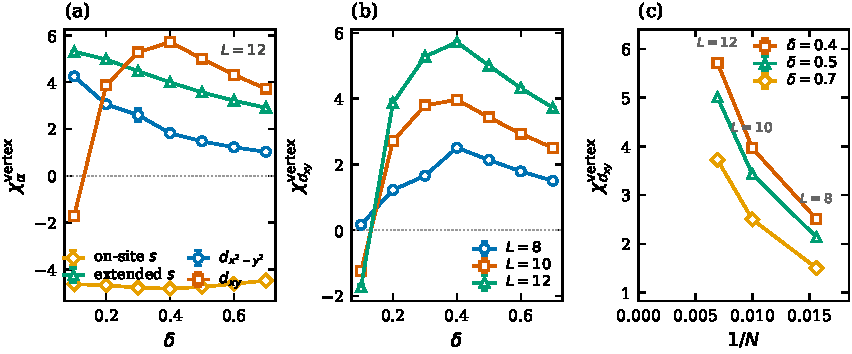
\includegraphics[width=\textwidth]{figures/fig09_pairing_fss}
\caption{Time-integrated pairing vertex at half filling. (a) the four channels at $L=12$ and $U=4$, (b) the $d_{xy}$ vertex against $\delta$ for $L=8$, $10$ and $12$, and (c) the same quantity against $1/N$. The vertex is the interaction-induced part of the pair-field correlator and vanishes identically at $U=0$ in all four channels. $d_{xy}$ grows with system size at every interaction strength studied.}
\label{fig:fig09_pairing_fss}
\end{figure*}

\begin{figure*}[tp]
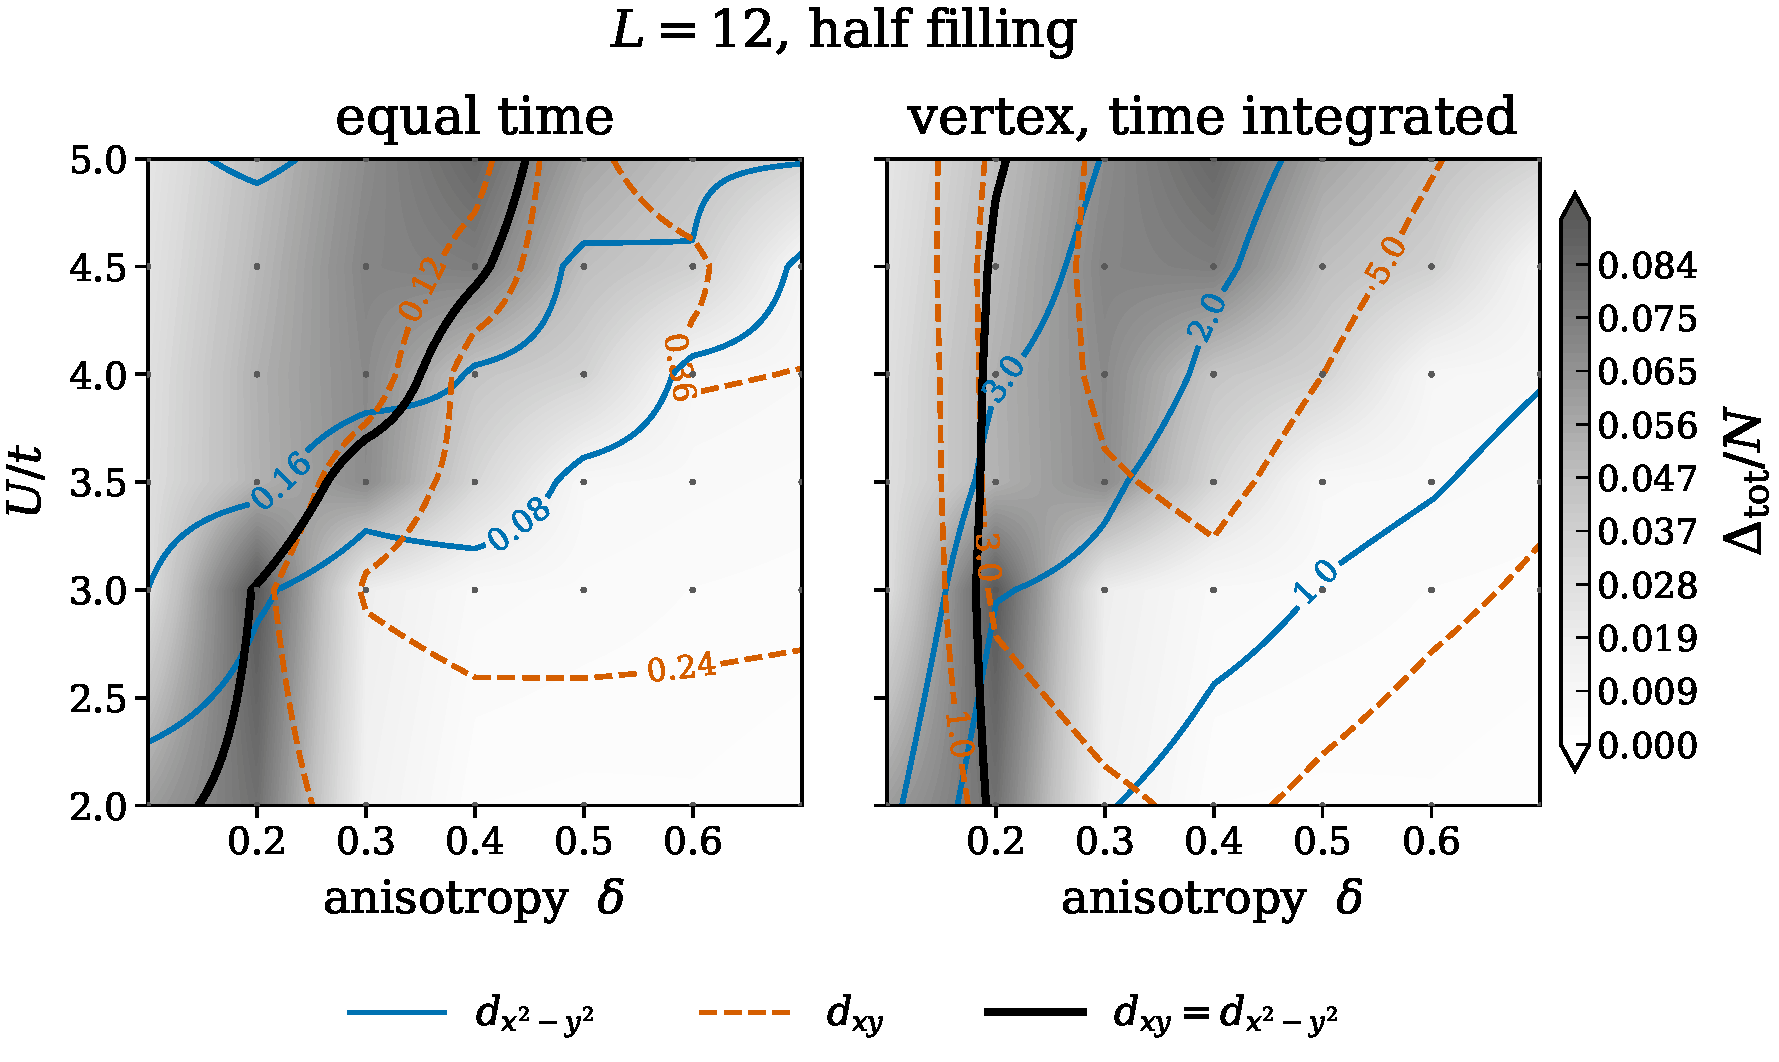
\includegraphics[width=\textwidth]{figures/fig_dchannels_eqtime_vs_vertex}
\caption{The two $d$ channels measured equal time (left) and time integrated (right) at $L=12$. The equal-time correlator carries a large uncorrelated part, so the vertex is the measure used for the claims in the text.}
\label{fig:fig_dchannels_eqtime_vs_vertex}
\end{figure*}

\begin{figure}[htbp]
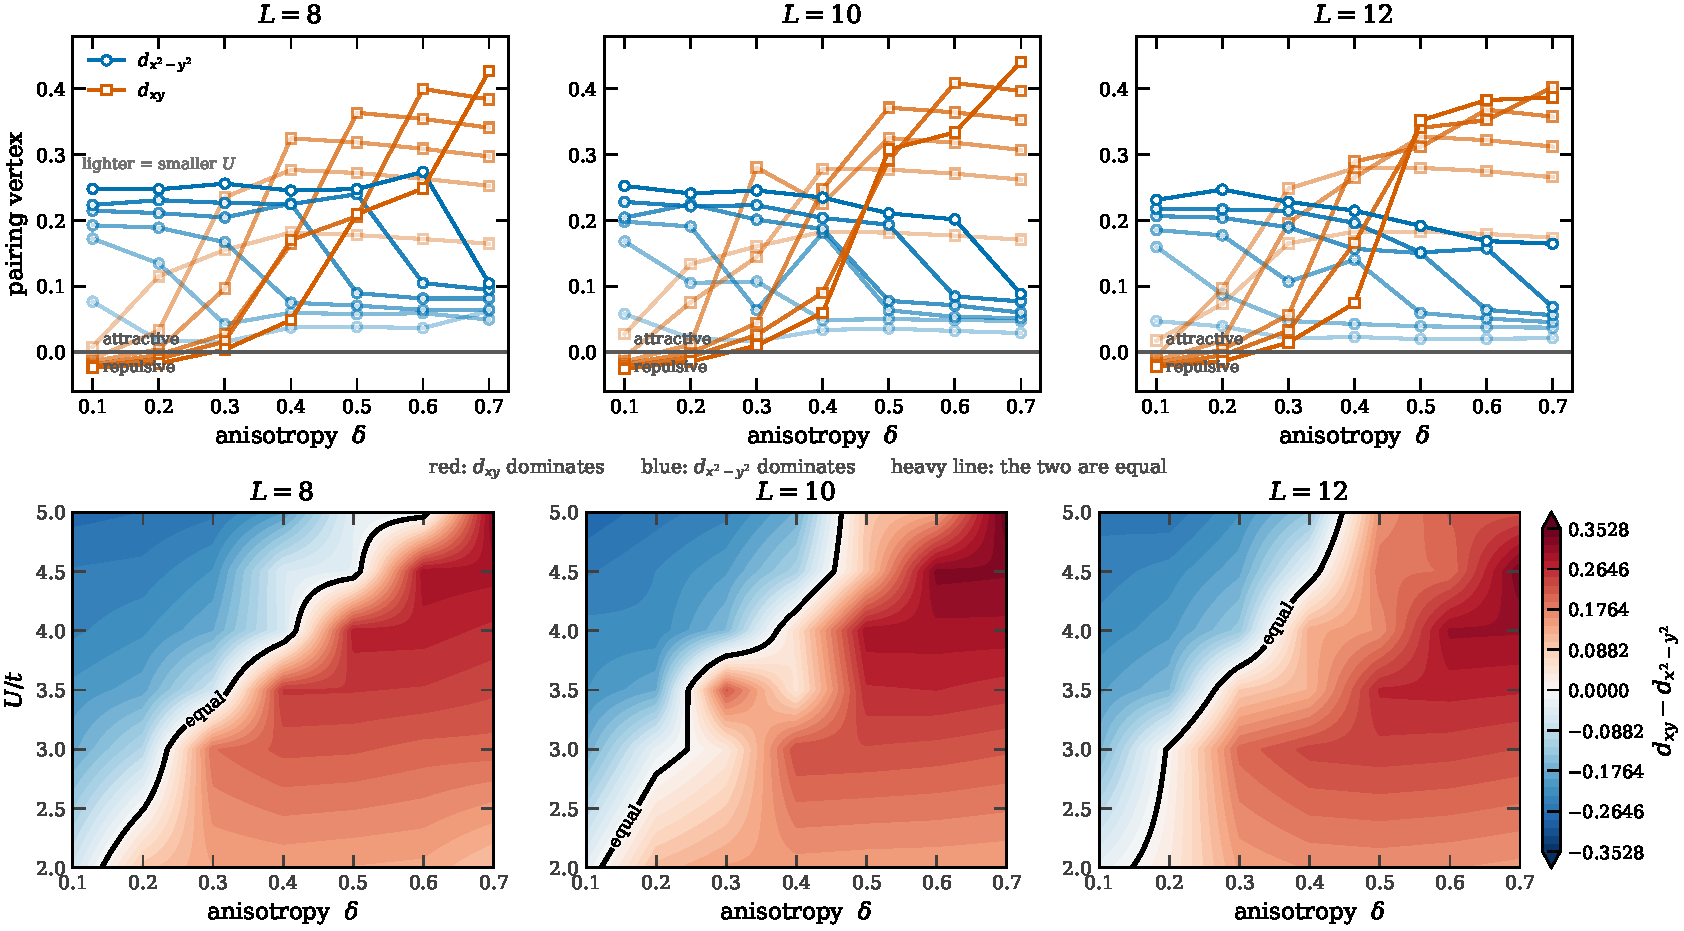
\includegraphics[width=\columnwidth]{figures/fig_d_channels_together}
\caption{Both $d$ channels in the $(U,\delta)$ plane at $L=12$. $d_{x^2-y^2}$ is positive everywhere, so it is never repulsive even where it is subdominant, and $d_{xy}$ is the larger of the two above $\delta\simeq0.19$.}
\label{fig:fig_d_channels_together}
\end{figure}

\begin{figure}[htbp]
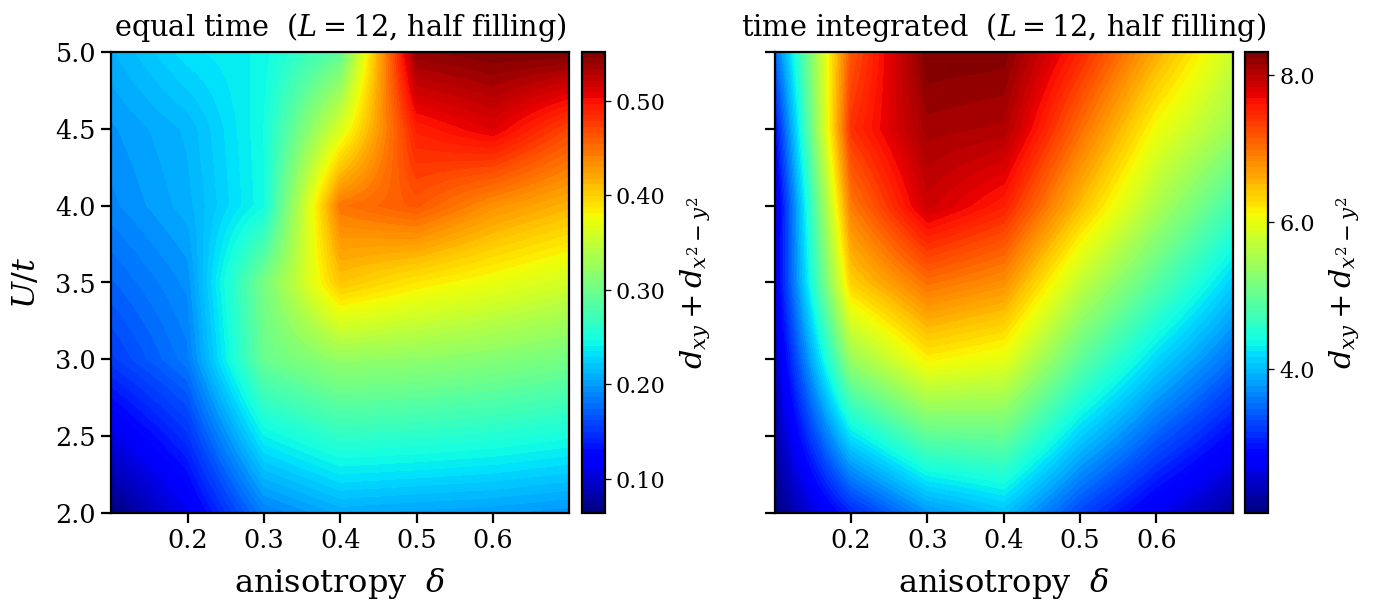
\includegraphics[width=\columnwidth]{figures/fig_dsum_L12}
\caption{Sum of the $d_{xy}$ and $d_{x^2-y^2}$ vertices at $L=12$, showing the total weight carried by the two sign-changing channels.}
\label{fig:fig_dsum_L12}
\end{figure}

\begin{figure}[htbp]
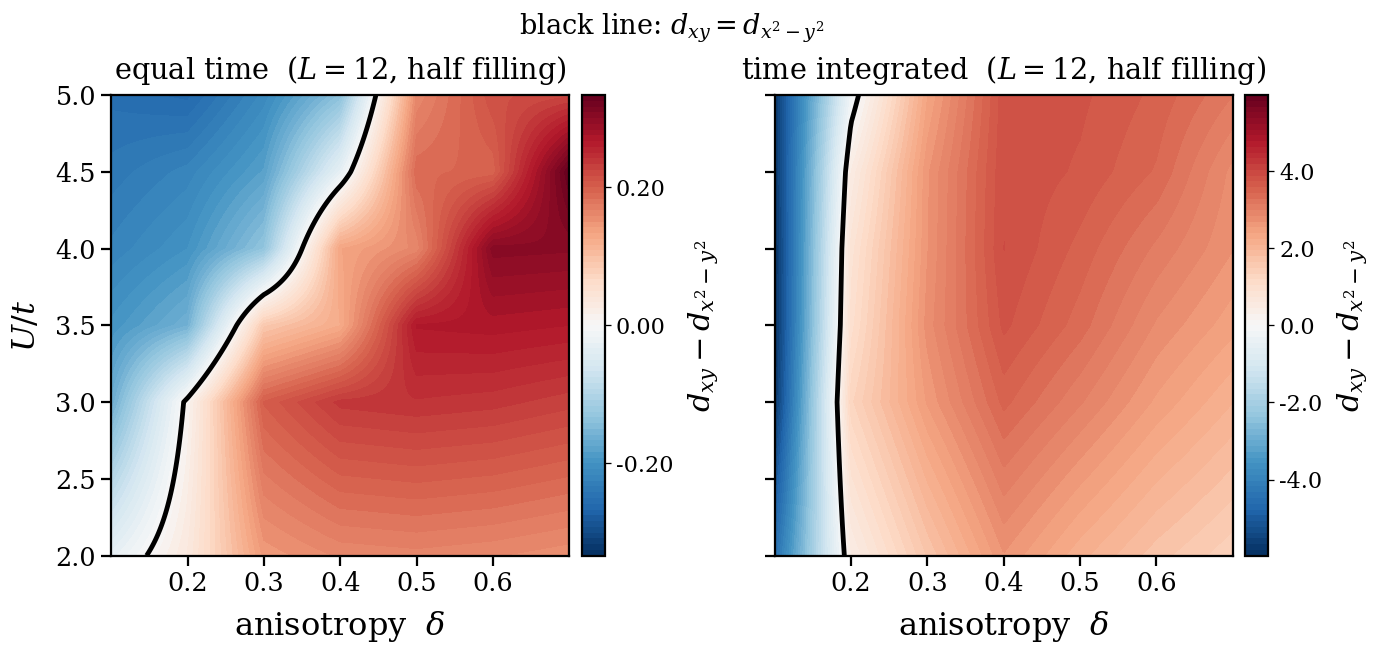
\includegraphics[width=\columnwidth]{figures/fig_ddiff_L12}
\caption{Difference of the $d_{xy}$ and $d_{x^2-y^2}$ vertices at $L=12$, on the same colour scale as the preceding figure.}
\label{fig:fig_ddiff_L12}
\end{figure}

% -------------------------------------------------------------------------
\section{Size dependence of the pairing vertex}
\label{sec:vertexfss}
% ---------------------------------------------------------------------------

The pairing vertex of Sec.~\ref{sec:pairing} was computed at $L = 8$, $10$, and
$12$ under identical settings, which allows the anisotropy of the channel
crossover to be followed with size.

The crossover anisotropy $\delta_c$, defined as the value at which the $d_{xy}$
vertex overtakes the extended $s$ vertex, is nearly independent of $U$ and
becomes more so as the lattice grows. Its spread across the six interaction
strengths studied is $0.148$ at $L = 8$, $0.049$ at $L = 10$, and $0.028$ at
$L = 12$, and the mean value moves from $0.235$ to $0.197$ to $0.192$. A
crossover that is set by the interaction strength would not converge in this
way, so we read $\delta_c \approx 0.19$ as a property of the lattice geometry.

The $d_{xy}$ vertex grows with system size at every interaction strength, by a
factor between $2.18$ and $2.38$ from $L = 8$ to $L = 12$. The $d_{x^2-y^2}$
vertex is positive in all $126$ cells at all three sizes, so that channel is
never repulsive even where it is subdominant. The optimal anisotropy for
$d_{xy}$ is $\delta = 0.4$ at essentially every size and interaction strength.

The two $d$ channels respond with opposite sign to the same change in
anisotropy at fixed interaction, so they are not simply rising and falling
together with the overall pairing scale.


\begin{figure*}[tp]
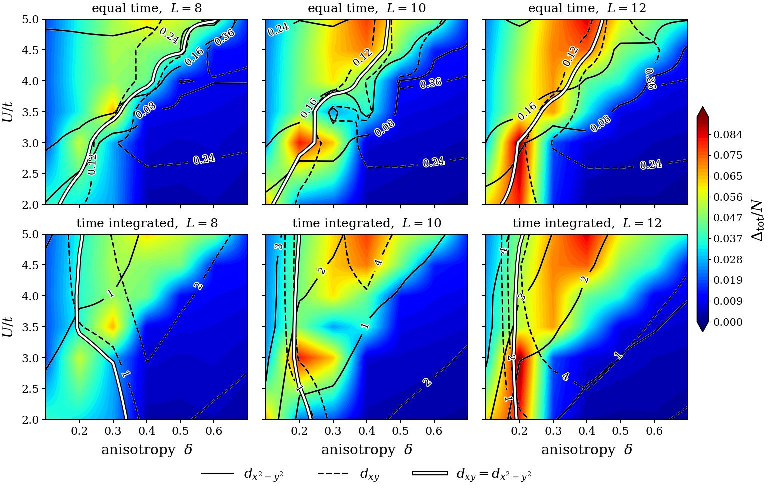
\includegraphics[width=\textwidth]{figures/fig_2row_eqtime_vertex_3L}
\caption{Equal-time pair correlator (top row) and time-integrated vertex (bottom row) for $L=8$, $10$ and $12$. The channel crossover straightens and its spread across $U$ narrows along the vertex row, which is the behavior expected of a quantity fixed by the lattice geometry rather than by the coupling.}
\label{fig:fig_2row_eqtime_vertex_3L}
\end{figure*}

\begin{figure*}[tp]
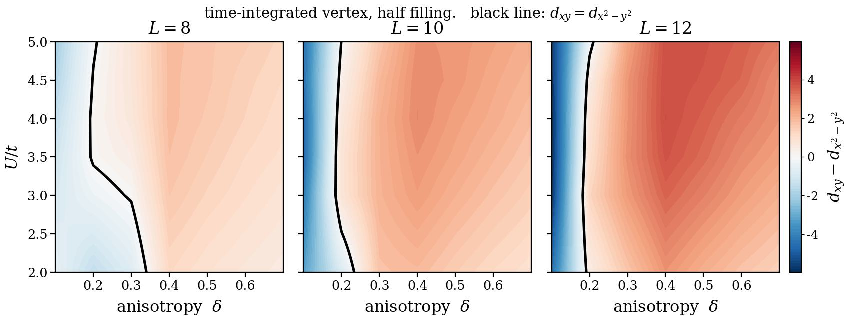
\includegraphics[width=\textwidth]{figures/fig_ddiff_vertex_3L}
\caption{Difference between the $d_{xy}$ and $d_{x^2-y^2}$ vertices over the $(U,\delta)$ plane at $L=8$, $10$ and $12$. The zero contour is the crossover anisotropy $\delta_c$, which is nearly flat in $U$ and whose spread across the interaction strengths studied falls from $0.148$ to $0.049$ to $0.028$ as the lattice grows.}
\label{fig:fig_ddiff_vertex_3L}
\end{figure*}

% -------------------------------------------------------------------------
\section{Robustness and comparison}
% ---------------------------------------------------------------------------

At half filling with periodic boundaries the noninteracting gap of
Eq.~(\ref{eq:H}) is zero at every $L$ and $\delta$ we examined, so the occupied
set is fixed by the trial state rather than by the spectrum. We repeated the
calculation with antiperiodic boundaries, which shift the momentum mesh off the
high-symmetry points and open a gap, at otherwise identical settings.


The closest published work is a determinant quantum Monte Carlo study of the
checkerboard Hubbard model that reports $d$-wave and $d + is$ pairing as the
dominant channels~\cite{Pan2024}. The two Hamiltonians are not the same. That
model keeps one diagonal per sublattice and omits the other, whereas
Eq.~(\ref{eq:H}) keeps both, and the two coincide only where our second diagonal
vanishes, at $\delta = t_1 = 0.3$. We verified that the single-particle spectra
agree there to within $4\times10^{-15}$.

At that point, and at half filling, we evaluated the vertex in the basis of
Ref.~\cite{Pan2024} alongside our own. Within their basis the $s$-wave channel
is the larger of the two at $U = 3$, $4$, and $4.5$. Including $d_{xy}$, which
their basis does not contain, gives a $d_{xy}$ vertex larger than either.
% data/pan, analyze_pan.py
The comparison is restricted, since Ref.~\cite{Pan2024} works at density
$n = 0.9$ and temperature $T/t = 1/6$ while our calculations are at half filling
in the ground state, and under the particle-hole transformation that relates the
two signs of the second-neighbor hopping their density maps to $n = 1.1$. The
statement is that the dominant channel we find lies outside the basis used
there, not that the two calculations disagree.


% -------------------------------------------------------------------------
\section{Conclusion}
The interaction-induced pairing vertex of the half-filled checkerboard Hubbard
model is zero in every channel at $U=0$ and is largest in the $d_{xy}$ channel
above an anisotropy $\delta_c \simeq 0.19$. The crossover is nearly independent
of the interaction strength and converges with system size, which identifies it
with the lattice geometry rather than with the coupling. The $d_{xy}$ vertex
grows with system size at every interaction strength studied, and $d_{x^2-y^2}$
is positive in all 126 cells examined and therefore never repulsive.

The dominant channel lies outside the basis used in the closest published
calculation on this lattice, so the comparison is one of basis rather than of
disagreement. Whether the $d_{xy}$ tendency survives to the thermodynamic limit
is not settled by the sizes reached here, and the constrained-path bias remains.

\appendix

% -------------------------------------------------------------------------
\section{Trial wave function and the selection of the constrained path}
\label{app:trial}
% ---------------------------------------------------------------------------

The constrained-path approximation replaces the sign problem with a bias fixed
by the trial wave function, so the trial is part of the method rather than an
implementation detail. We take the trial from an unrestricted Hartree-Fock
solution of Eq.~(\ref{eq:H}) at the same $U$, $\delta$, and filling, and we
select among the solutions reached from different starting densities by the
variational energy
\begin{equation}
E_{\mathrm{HF}} = \mathrm{Tr}\,(K \rho_{\uparrow}) + \mathrm{Tr}\,(K \rho_{\downarrow})
                + U \sum_i \langle n_{i\uparrow}\rangle \langle n_{i\downarrow}\rangle ,
\label{eq:ehf}
\end{equation}
with $\rho_{\sigma} = V_{\sigma} V_{\sigma}^{\dagger}$ built from the occupied
columns of the mean-field eigenvectors and $K$ the one-body matrix of
Eq.~(\ref{eq:H}).

Equation~(\ref{eq:ehf}) is not interchangeable with the sum of mean-field
eigenvalues. Each eigenvalue already contains the mean field of the opposite
spin, so that sum counts the interaction twice and orders competing solutions
differently from the energy. The two criteria can select different states, and
because the constrained path is fixed by whichever state is chosen, the
selection propagates into every measured quantity.

The size of the effect is not small. Selecting by the eigenvalue sum instead of
Eq.~(\ref{eq:ehf}) changes the trial in a substantial fraction of parameter
sets, and at half filling the state chosen that way carries the larger staggered
moment in every case where the two differ. We therefore report results obtained
with Eq.~(\ref{eq:ehf}) throughout.

The identity $E_{\mathrm{HF}} = \sum_p \varepsilon_p - U \sum_i \langle
n_{i\uparrow}\rangle \langle n_{i\downarrow}\rangle$ holds only at exact self
consistency and should not be substituted for Eq.~(\ref{eq:ehf}). A mean-field
iteration that mixes densities between steps does not reach that condition for
loosely converged solutions, which are precisely the ones whose ranking is at
issue.


% -------------------------------------------------------------------------
\section{Convergence in projection length}
\label{app:beta}
% ---------------------------------------------------------------------------

All results use a projection length $\beta = 32$ in units of $1/|t_0|$. Doubling
it to $\beta = 48$ at otherwise identical settings changes
$\Delta_{\mathrm{tot}}$ by between $0.1\%$ and $4.1\%$ with no systematic drift
in either direction, which we take as convergence.


% -------------------------------------------------------------------------
\section{Boundary conditions}
\label{app:bc}
% ---------------------------------------------------------------------------

At half filling with periodic boundaries the noninteracting spectrum of
Eq.~(\ref{eq:H}) is gapless at every $L$ and $\delta$ examined, so the occupied
set is fixed by the trial state rather than by the spectrum. Antiperiodic
boundaries shift the momentum mesh off the high-symmetry points and open a gap.

The sensitivity of the calculation to the momentum mesh was characterized on the
magnetic response rather than on the vertex. Its slope in $U$ agrees between the
two boundary conditions at $\delta = 0.1$ and at $\delta = 0.5$ and is ambiguous
at $\delta = 0.3$, where that slope passes through zero and its sign is most
sensitive to the mesh. We have not repeated the vertex calculation with
antiperiodic boundaries, so the mesh dependence of the pairing results is not
quantified here.

\begin{acknowledgments}
% TODO: funding and computing acknowledgments.
\end{acknowledgments}

\begin{thebibliography}{99}

% TODO: verify all bibliographic details before submission. Entries marked
% INCOMPLETE need the full reference supplied by the authors.

\bibitem{Smejkal2022a}
L.~\v{S}mejkal, J.~Sinova, and T.~Jungwirth,
Phys. Rev. X \textbf{12}, 031042 (2022).

\bibitem{Smejkal2022b}
L.~\v{S}mejkal, J.~Sinova, and T.~Jungwirth,
Phys. Rev. X \textbf{12}, 040501 (2022).

\bibitem{Kaushal2025}
N.~Kaushal and M.~Franz,
Phys. Rev. Lett. \textbf{135}, 156502 (2025).

\bibitem{Duerrnagel2025}
M.~D\"urrnagel \textit{et al.},
Phys. Rev. Lett. \textbf{135}, 036502 (2025);
arXiv:2412.14251.

\bibitem{Pan2024}
Y.~Pan, R.~Ma, C.~Chen, Z.~Jia, and T.~Ma,
arXiv:2409.16523.

\bibitem{OurPRB}
% INCOMPLETE: this is the group's published PRB defining Eq. (3). Full
% reference to be supplied by the authors.
[Authors], Phys. Rev. B \textbf{[vol]}, [page] ([year]).

\end{thebibliography}

\end{document}
